\documentclass[10pt,a4paper]{article}

\usepackage[margin=0.7in,top=0.65in,bottom=0.7in]{geometry}
\usepackage{amsmath,amssymb}
\usepackage{booktabs}
\usepackage[expansion=false]{microtype}
\usepackage{enumitem}
\usepackage{xurl}
\usepackage[hidelinks]{hyperref}
\usepackage{pgfplots}
\pgfplotsset{compat=1.16}
\usepackage{caption}
\captionsetup{font=small,labelfont=bf}
\usepackage{graphicx}

\usepackage{titlesec}
\titlespacing*{\section}{0pt}{5pt}{2pt}
\titlespacing*{\subsection}{0pt}{4pt}{1pt}
\titlespacing*{\paragraph}{0pt}{3pt}{6pt}
\titleformat*{\section}{\large\bfseries}
\titleformat*{\subsection}{\normalsize\bfseries}
\setlength{\textfloatsep}{6pt}
\setlength{\intextsep}{6pt}
\setlength{\abovecaptionskip}{3pt}
\setlength{\belowcaptionskip}{2pt}
\setlist{nosep,leftmargin=*}
\setlength{\parskip}{1pt}
\setlength{\parindent}{0pt}
\raggedbottom
\setlength{\emergencystretch}{2em}

\begin{document}

% ---------- Title Page ----------
\begin{titlepage}
\centering
\vspace*{1.2cm}

\IfFileExists{images/iitd.png}{{
\includegraphics[width=4.2cm]{images/iitd.png}}}{}

\vspace{1.0cm}

{\huge\scshape Indian Institute of Technology Delhi\par}

\vspace{0.4cm}

{\Large COL764: Information Retrieval and Web Search\par}

\vspace{2.2cm}

{\rule{0.85\textwidth}{0.8pt}\par}
\vspace{0.6cm}
{\LARGE\bfseries Assignment 3: Rank Fusion and Learning to Rank\par}
\vspace{0.6cm}
{\rule{0.85\textwidth}{0.8pt}\par}

\vspace{2.5cm}

\begin{minipage}{0.45\textwidth}
\centering
{\Large\bfseries Submitted by}\par
\vspace{0.25cm}
{\Large Aditya Anand\par}
{\Large 2023CS50284\par}
\end{minipage}%
\begin{minipage}{0.45\textwidth}
\centering
{\Large\bfseries Instructor}\par
\vspace{0.25cm}
{\Large Prof.\ Srikanta Bedathur\par}
\end{minipage}

\vfill

{\Large \today\par}

\vspace{1cm}

\end{titlepage}

% ---------- Report content begins ----------
\newpage

\section{Rank fusion}

\texttt{fuse\_candidates} combines four base rankers already computed in the MSLR features: BM25 on the whole document, BM25 on the title, LMIR.DIR on the whole document, and LMIR.JM on the whole document. The four scores are not on one scale, so CombSUM and CombMNZ min--max normalise each channel inside the query before adding. A channel whose values are all equal becomes all zeros and drops out. Ranks for RRF are 1-based, and a tie keeps the candidate order.
\[
\mathrm{RRF}(d)=\sum_s\frac{1}{c+\mathrm{rank}_s(d)},\quad
\mathrm{CombSUM}(d)=\sum_s\tilde s(d),\quad
\mathrm{CombMNZ}(d)=\mathrm{CombSUM}(d)\cdot|\{s:\tilde s(d)>0\}|.
\]
$\tilde s$ is the min--max score. CombMNZ counts a channel only when that normalised score is strictly positive. All three functions are in \texttt{submission/fusion.py}.

The submitted rule is \textbf{CombSUM of the first three channels}. On the 6{,}000 TRAIN queries a weight search kept BM25 on the whole document at weight 1 and tried $\{0, 0.25, 0.5, 1, 2\}$ on the other three. That search set LMIR.JM to 0, and the three-channel sum scores 0.3000. Equal-weight fusion of all four channels is lower on the same queries: CombSUM 0.2961, CombMNZ 0.2958, and RRF 0.2937 at its best constant $c=150$. The RRF grid included $c=60$. On DEV the submitted fusion scores nDCG@10 0.3105 and MAP@10 0.1302. DEV was only printed. The choice was made on TRAIN. Fusion uses no labels. It is the unsupervised baseline, and it sees 4 of the 136 features.

\section{Pointwise, pairwise, and LambdaMART}

The pointwise model is one hidden layer of 64 units. The loss is the squared error between the score and the relevance label, which is an integer from 0 to 4. Each document is its own training row. The loss does not know which other documents belong to the same query, and a mistake at rank 1 costs the same as a mistake at rank 50.

The pairwise model is three hidden layers of 256 units, the largest plain network Track~P accepts. The checked loss is RankNet. For a pair where document $i$ has the higher grade, the loss is $\log(1+\exp(-(s_i-s_j)))$, computed with \texttt{logaddexp} so a badly ordered pair does not overflow. Pairs are taken inside one query only, ties are dropped, and the higher grade comes first. During training, pairs are drawn with probability proportional to the grade gap, at most 4{,}000 per query, and each pair is multiplied by $|\Delta\mathrm{nDCG}|$ under the current scores. The gain is $2^y-1$, the discount is $1/\log_2(1+\mathrm{rank})$, and the change is divided by the query's ideal DCG@10. A swap near the top of the list gets a larger step than a swap of two irrelevant documents. The graded \texttt{ranknet\_loss} itself stays unweighted. Features are clipped to the 1st and 99th percentile of the training rows and then standardised. The standardizer is fit on the training rows only.

Both neural models train on a fixed $9/10$ of the TRAIN queries and early-stop on the other tenth, from \texttt{grouped\_kfold} with $k=10$ and seed 0. The saved weights are the ones with the best nDCG@10 on that tenth. DEV is scored once, after training.

LambdaMART is LightGBM's \texttt{lambdarank} objective. It uses the same pairwise gradient as RankNet and multiplies it by the change in nDCG from swapping the pair. That product is the lambda. A regression tree is fit to the lambdas, added with a learning rate, and the scores and lambdas are then recomputed. The shipped model has 2{,}835 trees and 127 leaves. It was continued from one stage to the next, with the learning rate falling from 0.05 to 0.015. Every stage was fit on TRAIN and DEV together, with no early stopping.

Each of the 136 features is stored together with its percentile inside the query and its z-score inside the query, 408 columns. \texttt{rerank\_with\_ltr} rebuilds the two extra blocks at scoring time. A percentile does not change if the feature is rescaled by an increasing function. A within-query z-score does not change if the feature is shifted or multiplied by a positive constant. Training also stacks changed copies of the rows, with new query ids so two copies of one query are not mixed in one percentile. The copies are Gaussian noise, multiplicative noise, a $\log(1+|x|)$ view, cells set to zero, cells set to missing, the five fields of a feature group shuffled, one or two fields zeroed, and a per-query rescaling. Labels are copied unchanged.

\begin{center}
\small
\begin{tabular}{lcc}
\toprule
Model & DEV nDCG@10 & DEV queries in the fit \\
\midrule
Pointwise & 0.4225 & no \\
Pairwise & 0.4550 & no \\
LambdaMART & 0.7079 & yes \\
\bottomrule
\end{tabular}
\end{center}

Pairwise is above pointwise because it trains on order inside the query and puts more weight on pairs that move nDCG@10. The LambdaMART number is higher still because those DEV queries were part of the fit. The cross-validation below is the score on queries the trees have not seen.

\section{Cross-validation and the gap}

I do not have the held-out queries, so the gap is measured by grouped 5-fold cross-validation inside TRAIN. All documents of a query go to the same fold. Splitting by row would put documents from one query on both sides and make the validation score look too high. For each fold the model trains on the other four. nDCG@10 is read at tree counts $100, 200, 300, 500, 750, 1000, 1500, 2000$ from the prefix of one run, so the reported fold is not used to decide when to stop. For each setting the number I keep is the tree count with the highest mean validation score. The figure is the leaf sweep: learning rate 0.05, at least 100 rows in a leaf, column sample 0.8. The four points use 1000, 300, 500 and 200 trees.

\begin{figure}[ht]
\centering
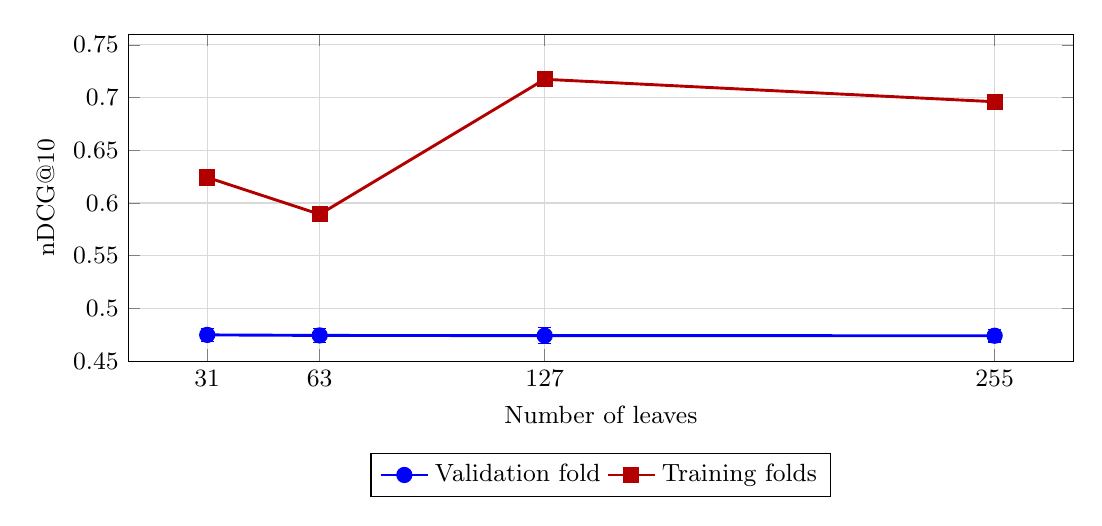
\begin{tikzpicture}
\begin{axis}[
  width=12.0cm, height=4.15cm, scale only axis,
  xlabel={Number of leaves},
  ylabel={nDCG@10},
  ymin=0.45, ymax=0.76,
  ytick={0.45,0.50,0.55,0.60,0.65,0.70,0.75},
  xtick={31,63,127,255},
  tick label style={font=\small},
  label style={font=\small},
  axis line style={black},
  grid=both,
  major grid style={gray!30},
  legend style={font=\small, draw=black, fill=white,
                at={(0.5,-0.28)}, anchor=north, legend columns=2},
  legend cell align=left,
  every axis plot/.append style={line width=1.05pt, mark size=2.4pt},
]
\addplot[color=blue, mark=*, error bars/.cd, y dir=both, y explicit]
  coordinates {
    (31,0.4749) +- (0,0.0059)
    (63,0.4744) +- (0,0.0063)
    (127,0.4742) +- (0,0.0077)
    (255,0.4741) +- (0,0.0059)
  };
\addlegendentry{Validation fold}
\addplot[color=red!70!black, mark=square*] coordinates {
  (31,0.6243) (63,0.5893) (127,0.7174) (255,0.6961)
};
\addlegendentry{Training folds}
\end{axis}
\end{tikzpicture}
\caption{Grouped 5-fold nDCG@10 on TRAIN against the number of leaves. Error bars are the standard deviation across the five folds.}
\end{figure}

\begin{center}
\footnotesize
\begin{tabular}{lrrrrr}
\toprule
lr / leaves / min leaf / columns & Trees & Val nDCG@10 & Train & Val/train \\
\midrule
0.05 / 31 / 100 / 0.8 & 1000 & $0.4749 \pm 0.0059$ & 0.6243 & 0.761 \\
0.05 / 63 / 100 / 0.8 & 300 & $0.4744 \pm 0.0063$ & 0.5893 & 0.805 \\
0.05 / 127 / 100 / 0.8 & 500 & $0.4742 \pm 0.0077$ & 0.7174 & 0.661 \\
0.05 / 255 / 100 / 0.8 & 200 & $0.4741 \pm 0.0059$ & 0.6961 & 0.681 \\
0.05 / 63 / 500 / 0.5 & 500 & $0.4741 \pm 0.0068$ & 0.6233 & 0.761 \\
0.025 / 63 / 500 / 0.5 & 1000 & $0.4766 \pm 0.0070$ & 0.6249 & 0.763 \\
0.0125 / 63 / 500 / 0.5 & 2000 & $0.4771 \pm 0.0068$ & 0.6263 & 0.762 \\
\bottomrule
\end{tabular}
\end{center}

The $\pm$ is the standard deviation of the five validation folds. \textbf{Validation stays inside 0.474 to 0.477} on every row. The training score does not. At 127 leaves it is 0.717 and the ratio falls to 0.661. The best ratio is 0.805, at 63 leaves and 300 trees, and that validation score is only 0.0005 below the 31-leaf run. The last three rows keep the tree shape fixed and spend more trees at a smaller learning rate. Validation rises by 0.003, from 0.4741 to 0.4771, which is smaller than the fold standard deviation of about 0.007, and the ratio stays near 0.76. The best clean estimate is that last row: 0.4771 on TRAIN queries the model did not fit, against 0.6263 on the queries it did fit.

That 0.477 sits next to the pairwise DEV score of 0.4550 and above the pointwise score of 0.4225. \textbf{The shipped DEV score of 0.7079 is an in-training score}, in the same band as the training-fold scores in the figure, because those DEV queries were in the fit. \textbf{0.477 is the local estimate} of nDCG@10 on unseen MSLR queries.

More leaves do not raise validation nDCG on clean features, so the shipped run does not use a deeper tree to chase that number. It keeps 127 leaves and spends the 2{,}835 trees on the corrupted copies and the within-query columns, with column sample 0.5, row bagging 0.9, L2 0.1, and a minimum leaf size of 20 or 40. The learning rate falls from 0.05 to 0.015 across the stages. The early stages mix a clean copy with moderate noise, a log view, shuffled fields and some zeroed cells. Later stages drop the clean copy, raise the noise, set cells to missing, and zero one or two fields. The last stage is 250 clean trees. Those copies are for the hidden robustness test: the same model is applied there with no retraining, and I do not know how the hidden versions are built. Noise, missing cells, dropped fields and rescaling are the changes I can train for, and the percentile and z-score columns stay put when a feature is rescaled.

\begin{center}
\small
\begin{tabular}{llll}
\toprule
Model & Trained on & Tuned on & Early stopping \\
\midrule
LambdaMART & TRAIN and DEV & 5-fold CV on TRAIN & none \\
Pointwise & 9/10 of TRAIN & not tuned & the other 1/10 of TRAIN \\
Pairwise & 9/10 of TRAIN & a TRAIN slice & the other 1/10 of TRAIN \\
Recipe & each benchmark's train and vali & the size rules above & that benchmark's vali, then a refit \\
\bottomrule
\end{tabular}
\end{center}

The pairwise sampling and learning rate were chosen on a TRAIN slice. The early-stopping tenth is also TRAIN, so the pairwise DEV score is on queries that model did not train on.

For the two undisclosed benchmarks the MSLR file cannot be reused, because the features are different and unnamed, and there may be up to about 300 of them. \texttt{recipe.py} trains up to six LambdaMART models and writes one file whose score is their average, by placing the trees in order and dividing every leaf value by the number of models. Three models see the raw columns and three also see the within-query percentile and z-score. The tree shapes are the size rule, twice the leaves, half the leaves, and a narrower column sample. A model is skipped when the time estimate says it will not fit in 20 minutes. Each model that runs stops early on that benchmark's validation file and is then refit on the training and validation rows together. With $n$ training rows and $d$ columns in the input that model sees, the number of leaves grows with $\sqrt{n}$ and is clipped to $[7,63]$, the minimum leaf size is $n/4000$ clipped to $[20,200]$, and the column sample shrinks as $d$ grows, down to 0.5. L2 is 10 when $n<50{,}000$ and 1 otherwise. Nothing in the recipe hard-codes 136 features.

\section{Leaves on the transfer track}

Track~C2 applies the shipped file with no retraining, so there is no second leaf sweep to plot for it. Track~C1 is different. \texttt{recipe.py} never sees the benchmark in advance, so the leaf count is a function of the file. With $n$ training rows,
\[
\mathrm{leaves}=\mathrm{clip}\bigl(2^{\mathrm{round}(\log_2(\sqrt{n}/16))}-1,\; 7,\; 63\bigr).
\]
Two of the six models then move off that value: the deep model uses $2\cdot\mathrm{leaves}+1$, and the shallow model uses half of it. The figure is that rule. It is not an nDCG curve. The hidden files are not available, so the plot is the leaf count the recipe would actually train.

\begin{figure}[ht]
\centering
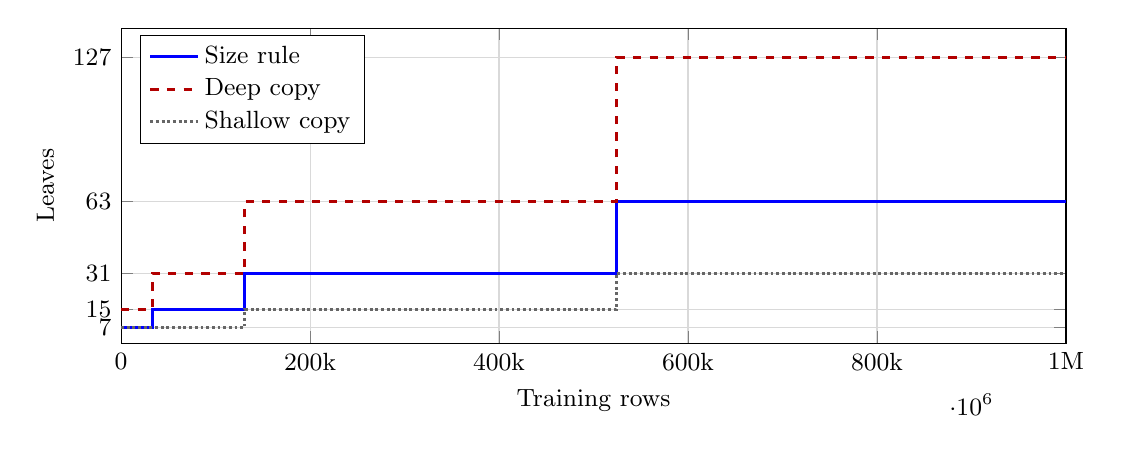
\begin{tikzpicture}
\begin{axis}[
  width=12.0cm, height=4.0cm, scale only axis,
  xlabel={Training rows},
  ylabel={Leaves},
  xmin=0, xmax=1000000,
  ymin=0, ymax=140,
  xtick={0,200000,400000,600000,800000,1000000},
  xticklabels={0,200k,400k,600k,800k,1M},
  ytick={7,15,31,63,127},
  tick label style={font=\small},
  label style={font=\small},
  axis line style={black},
  grid=both,
  major grid style={gray!30},
  legend style={font=\small, draw=black, fill=white,
                at={(0.02,0.98)}, anchor=north west, legend columns=1},
  legend cell align=left,
  every axis plot/.append style={line width=1.05pt},
]
\addplot[color=blue] coordinates {
  (0,7) (32768,7) (32768,15) (131072,15) (131072,31) (524288,31) (524288,63) (1000000,63)
};
\addlegendentry{Size rule}
\addplot[color=red!70!black, dashed] coordinates {
  (0,15) (32768,15) (32768,31) (131072,31) (131072,63) (524288,63) (524288,127) (1000000,127)
};
\addlegendentry{Deep copy}
\addplot[color=black!60, densely dotted] coordinates {
  (0,7) (131072,7) (131072,15) (524288,15) (524288,31) (1000000,31)
};
\addlegendentry{Shallow copy}
\end{axis}
\end{tikzpicture}
\caption{Leaves chosen by \texttt{recipe.py} from the number of training rows. The steps are where the formula changes: 32{,}768, 131{,}072 and 524{,}288 rows. Full MSLR TRAIN plus DEV, about 958{,}000 rows, falls in the top step: 63, 127 and 31 leaves.}
\end{figure}

Below 32{,}768 rows every model is kept at 7 or 15 leaves, and L2 is 10 until 50{,}000 rows. The minimum leaf size is 20 until 80{,}000 rows and then rises as $n/4000$, hitting the cap of 200 at 800{,}000 rows. The column sample depends on the width, not on the rows: it is 1.0 at 32 columns, about 0.69 at 136 columns, and 0.50 at 300 columns. A full recipe run on MSLR TRAIN plus DEV took 313 seconds and 4.0\,GB. A synthetic file at the stated limit, 500{,}000 rows and 300 features, took 353 seconds and 5.2\,GB.

\section{Final configuration}

\textbf{Fusion is the three-channel CombSUM.} The pointwise and pairwise networks are trained only on TRAIN and stopped on a TRAIN fold. \textbf{The LambdaMART file has 2{,}835 trees and 127 leaves}, is fit on TRAIN and DEV, and is trained on the within-query columns and the corrupted copies. The 63-leaf clean run has the better validation-to-train ratio, 0.805, with the same validation score near 0.477. I kept the longer run so the extra trees see noisy, missing and rescaled rows. \textbf{The DEV score of 0.7079 is an in-training score. The score I use for unseen queries is about 0.477.}

\section{AI use and code provenance}

\paragraph{AI use.}
I used Claude Code (Anthropic, Claude Opus 5.5) and Cursor (Grok) to read the starter code, write the submission, run the experiments and draft this report. I chose the fusion channels, the LambdaMART settings and the recipe rules, and I checked the numbers. I am responsible for the submission.

\paragraph{Code provenance.}
No external code was copied. RRF follows Cormack, Clarke and Buettcher (SIGIR, 2009). CombSUM and CombMNZ follow Fox and Shaw (TREC-2, 1994). RankNet follows Burges et al.\ (ICML, 2005). The $|\Delta\mathrm{nDCG}|$ weights follow Burges (MSR-TR-2010-82) and are applied only outside the graded \texttt{ranknet\_loss}. LambdaMART is LightGBM's \texttt{lambdarank} objective. The libraries are NumPy, LightGBM and PyTorch.

\end{document}
